\documentclass[conference]{IEEEtran}
\IEEEoverridecommandlockouts

\usepackage{cite}
\usepackage{amsmath,amssymb,amsfonts}
\usepackage{algorithmic}
\usepackage{graphicx}
\usepackage{textcomp}
\usepackage{xcolor}
\usepackage{booktabs}
\usepackage{multirow}
\usepackage{tikz}
\usetikzlibrary{arrows.meta, positioning, shapes.geometric, fit, backgrounds}
\usepackage{url}
\usepackage{hyperref}
\hypersetup{colorlinks=false}

\def\BibTeX{{\rm B\kern-.05em{\sc i\kern-.025em b}\kern-.08em
    T\kern-.1667em\lower.7ex\hbox{E}\kern-.125emX}}

\begin{document}

\title{Markov-Initialized Transformers for Explainable\\
Android Malware Family Classification}

\author{
\IEEEauthorblockN{Arav Jain}
\IEEEauthorblockA{\textit{Department of Applied Mathematics}\\
\textit{Delhi Technological University}\\
aravjain.int@urbancompany.com}
\\[0.2cm]
\IEEEauthorblockN{Divyanshu Bansal}
\IEEEauthorblockA{\textit{Department of Applied Mathematics}\\
\textit{Delhi Technological University}\\
divyanshubansal\_mc22a14\_03@dtu.ac.in}
\and
\IEEEauthorblockN{Harij Sharma}
\IEEEauthorblockA{\textit{Department of Applied Mathematics}\\
\textit{Delhi Technological University}\\
email address or ORCID}
\\[0.2cm]
\IEEEauthorblockN{Anshul Arora}
\IEEEauthorblockA{\textit{Department of Applied Mathematics}\\
\textit{Delhi Technological University}\\
email address or ORCID}
}

\maketitle

\begin{abstract}
Mobile malware sandboxes generate rich API call traces that capture true
runtime behavior, but the deep learning models that classify these traces
offer little insight into their decisions.
We explore whether embedding initialization can make a Transformer's own
attention mechanism more interpretable.
Our approach builds a global k-spaced API transition matrix
($k \in \{1,\ldots,10\}$), factorizes it via Truncated SVD, and uses
the resulting vectors to initialize the model's token embeddings before
any labeled training, encoding global behavioral structure into the
embedding space from the outset.
To measure the effect on transparency, we use a deletion test: if masking
the tokens that the \textit{[CLS]} attention map ranks highest causes a
larger confidence drop than masking random tokens, the attention is
meaningfully aligned with the model's actual decision.
Against a plain randomly-initialized Transformer on 9,337 Droidmon
execution traces across 8 Android malware families (3-fold stratified CV),
the Markov-initialized variant shows a substantially larger faithfulness
gap at $m{=}20$ (27.1\% vs.\ 17.0\%), at a modest 2.6\,pp Macro-F1
cost (0.858 vs.\ 0.884).
A per-family breakdown reveals that the gain is concentrated in families
with stereotyped API chains and absent for parasitic malware that blends
into host-app traffic, offering a principled account of where structural
initialization helps.
\end{abstract}

\begin{IEEEkeywords}
Android malware classification, Transformer, explainability,
Markov chain, API call sequences, attention faithfulness, deletion test
\end{IEEEkeywords}

% ─────────────────────────────────────────────────────────────────────────────
\section{Introduction}

Android malware continues to pose a significant threat to mobile security,
with over three million new malicious samples detected annually~\cite{av_test_2023}.
Family-level classification, attributing a sample to a specific malware
family such as Airpush, DroidKungFu, or Fusob, is essential for incident
response, threat intelligence, and understanding the behavioral evolution
of malware campaigns. The distinction is clinically meaningful: an
Airpush infection (unauthorized adware and user tracking) calls for
permission revocation and user notification, while a DroidKungFu
infection (root exploitation followed by credential exfiltration)
demands immediate device isolation, forensic chain-of-custody analysis,
and credential rotation. A classifier that identifies the family
provides actionable remediation context that binary detection cannot.

Dynamic analysis via sandboxing captures actual runtime API calls rather
than static bytecode, providing traces that are robust to code obfuscation.
Deep learning models, including CNNs, LSTMs, and Transformers, achieve
high accuracy on such traces but operate as black boxes. Post-hoc
explanation methods such as SHAP~\cite{lundberg2017shap} and LIME
explain a surrogate model, not the model itself. Intrinsic
explainability, where the model's own internal representations serve
as explanations, remains underexplored in the malware domain.

The \textit{[CLS]} token's attention distribution over input tokens
is a natural candidate for intrinsic explanation: it produces a
per-sample importance ranking without any external computation.
However, whether attention constitutes a \textit{faithful}
explanation, one that identifies the tokens the model genuinely
relies on, is empirically contested~\cite{jain2019attention,
wiegreffe2019attention}. Deletion tests~\cite{samek2017evaluating}
provide a concrete criterion that sidesteps the theoretical debate:
if masking the highest-attention tokens reduces model confidence
more than masking random tokens, the attention map has predictive
alignment with model behavior.

We propose to improve attention faithfulness by initializing the
Transformer's token embeddings from SVD-factorized Markov transition
matrices built from k-spaced API co-occurrences in the training set.
This injects global behavioral structure into the embedding space
before any labeled training begins. Our hypothesis is that embeddings
pre-encoded with transition dynamics will guide attention heads toward
behaviorally relevant tokens, producing more faithful explanations.

Our contributions are:
\begin{enumerate}
  \item A method for constructing Markov-initialized embeddings via SVD
    factorization of k-spaced API transition matrices, directly compatible
    with standard Transformer architectures.
  \item A controlled ablation on 9,337 samples demonstrating that this
    initialization produces measurably more faithful \textit{[CLS]}
    attention maps (+10.1\,pp faithfulness gap at $m{=}20$).
  \item A per-family faithfulness analysis revealing family-specific
    patterns and a principled discussion of the accuracy--explainability
    tradeoff.
\end{enumerate}

% ─────────────────────────────────────────────────────────────────────────────
\section{Related Work}

\subsection{Deep Learning for Malware Classification}
Early static-analysis work represented malware as grayscale bytecode
images and applied CNNs~\cite{nataraj2011malware}. Sequence-based models
using LSTMs and GRUs on API call traces showed strong generalization to
unseen variants~\cite{ye2019deep}. More recently, Transformer
architectures have been applied to API sequence classification, exploiting
self-attention to model long-range behavioral dependencies between API
calls. None of these works directly assess the faithfulness of the
resulting attention-based explanations.

\subsection{Explainability in Security ML}
Post-hoc methods such as SHAP and LIME have been applied to malware
classifiers~\cite{lundberg2017shap}, but they explain a surrogate model
rather than the trained model itself. Recent work in explainable Android malware detection has utilized post-hoc techniques; for example, Soi et al.~\cite{soi2024enhancing} apply SHAP to 1D-CNNs over API sequences, while Wu et al.~\cite{wu2021why} use input gradients for LSTMs. However, these methods typically focus on single-API attributions post-training. In contrast, our approach intrinsically encodes transition patterns directly into the embedding space.

The use of attention weights as
intrinsic explanations is theoretically contested: Jain and
Wallace~\cite{jain2019attention} show that alternative attention
distributions can yield identical predictions, undermining the claim
that attention reveals what the model relies on; Wiegreffe and
Pinter~\cite{wiegreffe2019attention} argue attention can still serve as
a partial explanation under different faithfulness definitions.
Deletion tests~\cite{samek2017evaluating} provide an empirical
faithfulness criterion that sidesteps this debate: they measure directly
whether the tokens a model attends to are the tokens it relies on.
Alternative intrinsic explanation methods include attention
rollout~\cite{abnar2020rollout}, which propagates attention through all
layers by composing the per-layer matrices and accounting for residual
connections, and gradient-based approaches such as Integrated
Gradients~\cite{sundararajan2017integrated}, which attribute output
changes to input features via path integration.
These methods can yield more accurate saliency maps in some settings but
require additional backward passes or multi-layer composition at
inference time. We use raw averaged CLS attention as our explanation
because it requires no additional computation and is directly
interpretable to practitioners; the deletion test then provides
empirical evidence of whether this simple explanation is meaningful.

\subsection{Graph-Based and Markov Approaches}
D'Angelo et al.~\cite{dangelo2023kspaced} model malware behavior as
k-spaced associative rules extracted from Droidmon API traces, achieving
strong interpretable classification on the same dataset we use.
GloVe~\cite{pennington2014glove} and Word2Vec~\cite{mikolov2013word2vec}
establish the broader precedent for deriving dense token embeddings from
co-occurrence matrix factorization. We are the first to bridge Markov
transition modeling with Transformer embedding initialization for malware
classification, and to measure the effect on attention faithfulness
directly via a deletion test.

% ─────────────────────────────────────────────────────────────────────────────
\section{Methodology}

\subsection{Preprocessing and Tokenization}
We use API call traces from the Droidmon dynamic analysis
sandbox~\cite{droidmon}. Each trace is a sequence of Android API events
recorded during sandboxed execution. We apply reflection-aware
tokenization: calls resolved via Java reflection are tagged
\texttt{REFL:class.method} to preserve the true call target rather than
collapsing to a generic reflection token.

A vocabulary is constructed over the training set with a minimum
frequency threshold of $f_{\min}=2$, yielding $|V|=1{,}118$ unique
API tokens plus special tokens PAD and UNK. Sequences are truncated to
$L_{\max}=512$ using \textit{head truncation} (retaining the first 512
tokens), selected via a sweep over $\{256, 512, 768\}$ with both head
and tail strategies; head truncation outperformed tail truncation by
1.7--2.9\,pp Macro-F1 at all tested lengths, indicating that early API
calls (SDK initialization, reflection setup, permission requests) carry
more family-discriminating signal.

\subsection{Transformer Architecture}
\label{sec:arch}

Our Transformer~\cite{vaswani2017attention} (Fig.~\ref{fig:arch})
prepends a learnable \textit{[CLS]} token to every input sequence and
classifies from the CLS final hidden state.

\textbf{Architecture.}
$d_{\text{model}}=128$, $H=4$ attention heads, $N_{\text{layers}}=2$
Transformer encoder layers, feed-forward dimension $d_{\text{ff}}=256$,
dropout $p=0.15$. Classification uses a two-layer MLP over the
$d_{\text{model}}$-dimensional CLS representation. Total parameters:
$\approx$515K.

\textbf{Loss.}
Class-weighted cross-entropy with inverse-frequency weights addresses
the 35$\times$ imbalance between Airpush (63\% of samples) and the
two smallest families.

\textbf{Explainability.}
For each sample, we collect the per-layer, per-head CLS attention row
$\mathbf{a}^{(\ell,h)}_{\text{CLS}} \in \mathbb{R}^{L+1}$
(the row of the softmax attention matrix corresponding to the CLS
position) and average across all heads and layers to obtain a single
importance vector $\hat{\mathbf{a}} \in \mathbb{R}^{L}$ over input
tokens. This serves as the intrinsic explanation without any
post-hoc computation.

\begin{figure}[t]
\centering
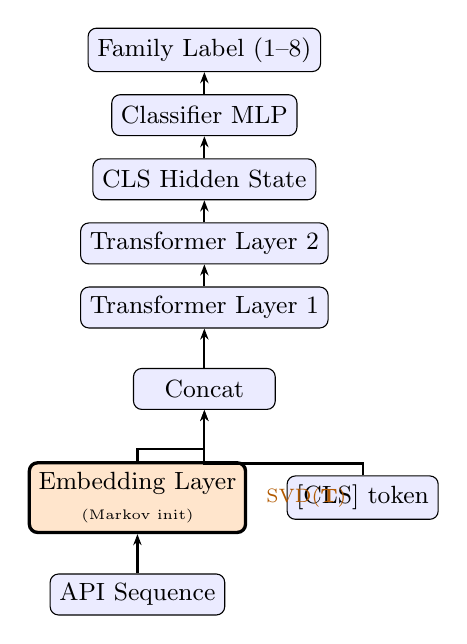
\begin{tikzpicture}[
  font=\small,
  box/.style={draw, rounded corners=3pt, minimum width=1.8cm,
              minimum height=0.52cm, align=center, fill=blue!8},
  boldbox/.style={draw, rounded corners=3pt, minimum width=1.8cm,
                  minimum height=0.52cm, align=center, fill=orange!20,
                  very thick},
  arr/.style={-{Stealth[length=4pt]}, thick},
  node distance=0.50cm and 0.0cm
]
  \node[box] (inp) {API Sequence};
  \node[boldbox, above=of inp] (emb) {Embedding Layer\\{\tiny (Markov init)}};
  \node[box, right=0.5cm of emb] (cls) {[CLS] token};
  \node[box, above=0.65cm of emb, xshift=0.85cm] (cat) {Concat};
  \node[box, above=of cat] (t1) {Transformer Layer 1};
  \node[box, above=0.28cm of t1] (t2) {Transformer Layer 2};
  \node[box, above=0.28cm of t2] (clsout) {CLS Hidden State};
  \node[box, above=0.28cm of clsout] (clf) {Classifier MLP};
  \node[box, above=0.28cm of clf] (out) {Family Label (1--8)};

  \draw[arr] (inp) -- (emb);
  \draw[arr] (cls.north) -- ++(0,0.15) -| (cat);
  \draw[arr] (emb.north) -- ++(0,0.15) -| (cat);
  \draw[arr] (cat) -- (t1);
  \draw[arr] (t1) -- (t2);
  \draw[arr] (t2) -- (clsout);
  \draw[arr] (clsout) -- (clf);
  \draw[arr] (clf) -- (out);

  \node[right=0.12cm of emb, font=\scriptsize, text=orange!70!black]
    {SVD($\mathbf{T}$)};
\end{tikzpicture}
\caption{Architecture. The embedding layer (orange) is initialized from
SVD-factorized Markov transition matrices in the proposed model.
Classification uses the CLS hidden state; CLS attention weights averaged
across all heads and layers form the intrinsic per-sample explanation.}
\label{fig:arch}
\end{figure}

\subsection{Markov Embedding Initialization}
\label{sec:markov}

\textbf{Transition matrix construction.}
For each training sequence $\mathbf{s} = (s_1, s_2, \ldots, s_n)$, we
extract all k-spaced pairs $(s_i, s_{i+k})$ for $k \in \{1,\ldots,10\}$
and accumulate a global count matrix:
\begin{equation}
  C(i,j) \mathrel{+}= 1
  \quad \forall k \in [1,10],\; \forall (s_i, s_{i+k}) \in \mathbf{s}.
\end{equation}
Aggregating over all training sequences yields
$\mathbf{C} \in \mathbb{R}^{|V| \times |V|}$. Row-normalizing gives the
transition matrix:
\begin{equation}
  T_{ij} = \frac{C_{ij}}{\sum_j C_{ij}}.
\end{equation}
The k-spacing range $[1,10]$ simultaneously captures local (adjacent)
and medium-range (contextual) co-occurrences, reflecting the multiscale
structure of malware behavioral patterns. A global matrix (rather than
per-class matrices) is used because class labels are unavailable at
inference time.

The left singular vectors $\mathbf{U}_d$ can be understood as a
low-rank approximation of the row space of $\mathbf{T}$: APIs with
similar outgoing transition profiles receive geometrically similar
embedding vectors, while APIs that tend to co-occur with a distinctive
set of partners receive distinctive representations. This means that
APIs belonging to the same behavioral chain (for example, the
telephony initialization, message composition, and send calls that
constitute the SmsPay SMS-fraud sequence) are embedded close together
in $\mathbb{R}^{d}$ before training begins, providing a natural
inductive bias toward attending to semantically coherent API groups.

\textbf{SVD factorization.}
We apply Truncated SVD to $\mathbf{T}$:
\begin{equation}
  \mathbf{T} \approx \mathbf{U}_d \boldsymbol{\Sigma}_d \mathbf{V}_d^\top,
  \quad \mathbf{U}_d \in \mathbb{R}^{|V| \times d_{\text{model}}},
\end{equation}
retaining $d_{\text{model}}=128$ singular components. Each row of
$\mathbf{U}_d$ encodes one API token's behavioral context as a
dense 128-dimensional vector. This factorization is analogous to
GloVe~\cite{pennington2014glove}, which derives embeddings from
co-occurrence matrix factorization; here the co-occurrence structure
encodes sequential transition dynamics across ten spacings simultaneously.

\textbf{Initialization.}
The rows of $\mathbf{U}_d$ are copied into the Transformer's
\texttt{nn.Embedding} layer as initial weights; the PAD embedding is
zeroed. The embedding layer is then frozen for 5 epochs---forcing
attention heads to learn to read the pre-encoded structure---before
unfreezing for end-to-end fine-tuning.

\subsection{Faithfulness Deletion Test}
\label{sec:deletion}

We evaluate whether the averaged CLS attention map $\hat{\mathbf{a}}$
faithfully identifies the tokens the model relies on for its prediction.
For each test sample $(\mathbf{x}, y)$:
\begin{enumerate}
  \item Compute baseline probability $P_0 = P(y \mid \mathbf{x})$.
  \item Rank tokens by descending $\hat{\mathbf{a}}$; select top-$m$
    indices $\mathcal{I}_{\text{attn}}$.
  \item Mask $\mathcal{I}_{\text{attn}}$ by replacing with PAD;
    re-run inference to obtain $P_{\text{attn}}$.
  \item Repeat with $m$ uniformly random indices to obtain $P_{\text{rand}}$.
\end{enumerate}
The \textit{faithfulness gap}
$G = (P_0 - P_{\text{attn}}) - (P_0 - P_{\text{rand}})$
measures how much more the model relies on its high-attention tokens
than on random ones. We evaluate at $m \in \{5, 10, 20\}$ and report
means over 30 samples per family (240 total). $G > 0$ is a necessary,
but not sufficient, condition for faithful explanation.

\subsection{Training Protocol}
Both the plain and Markov-initialized Transformers use identical
configurations: AdamW optimizer, learning rate $5 \times 10^{-4}$,
batch size 64, cosine annealing with $T_{\max}=100$ epochs, gradient
clipping at 1.0, and early stopping with patience 20 on validation Macro-F1.
We use 3-fold stratified cross-validation with the same fold assignments
and random seed (42) across all experiments to ensure fair comparison.
The SVD embedding dimension used is $d_{\text{model}}=128$.

% ─────────────────────────────────────────────────────────────────────────────
\section{Experimental Setup}
\label{sec:setup}

\subsection{Dataset}
We use the Droidmon execution traces from D'Angelo et
al.~\cite{dangelo2023kspaced}, obtained directly from the authors.
Samples with trace length $< 5$ API calls are excluded, yielding 9,337
traces across 8 malware families (Table~\ref{tab:dataset}). The corpus
exhibits a 35$\times$ class imbalance between the dominant family
(Airpush, 63\%) and the two smallest (Fusob and SmsPay, $<2\%$ each).
Class-weighted loss and stratified fold assignment mitigate this imbalance.

Our methodology relies on dynamic API traces, which capture runtime behavior and obfuscation resistance, differentiating it from static-feature datasets like Drebin~\cite{drebin2014} or CICAndMal2017~\cite{lashkari2018cicandmal2017}. However, evaluating on a single dataset remains a limitation; future work must verify generalization to other benchmarks.

\begin{table}[t]
\centering
\caption{Dataset: Droidmon traces from D'Angelo et al.~\cite{dangelo2023kspaced}.}
\label{tab:dataset}
\begin{tabular}{lrl}
\toprule
\textbf{Family} & \textbf{Samples} & \textbf{Primary Behavior} \\
\midrule
Airpush      & 5,880 & Aggressive adware, user tracking \\
DroidKungFu  & 1,257 & Root exploit, data exfiltration \\
Opfake       &   596 & SMS fraud, code packing \\
GinMaster    &   523 & Backdoor, privilege escalation \\
Jisut        &   430 & Ransomware + SMS fraud \\
Genpua       &   312 & Premium SMS fraud \\
SmsPay       &   173 & Premium SMS fraud \\
Fusob        &   166 & Ransomware \\
\midrule
\textbf{Total} & \textbf{9,337} & \\
\bottomrule
\end{tabular}
\end{table}

\subsection{Baselines}
We compare against: Random Forest~\cite{breiman2001rf} (100 trees),
LinearSVM, Decision Tree, Gaussian Na\"{i}ve Bayes (GNB), and a 2-layer
BiLSTM~\cite{hochreiter1997lstm} ($d=128$, mean-pooled). All classical
models use bag-of-API-ngrams features (TF-IDF) with identical class
weights; all neural models use the same sequence representation and
folds as the Transformers.

\subsection{Metrics}
We report Macro-F1 (primary), Accuracy, and Macro-AUROC as
mean\,$\pm$\,std over 3 folds. Macro-F1 averages per-class F1 scores
without weighting by support, preventing the dominant Airpush class
from masking minority-family performance.

% ─────────────────────────────────────────────────────────────────────────────
\section{Results and Discussion}

\begin{figure*}[tp]
\centering
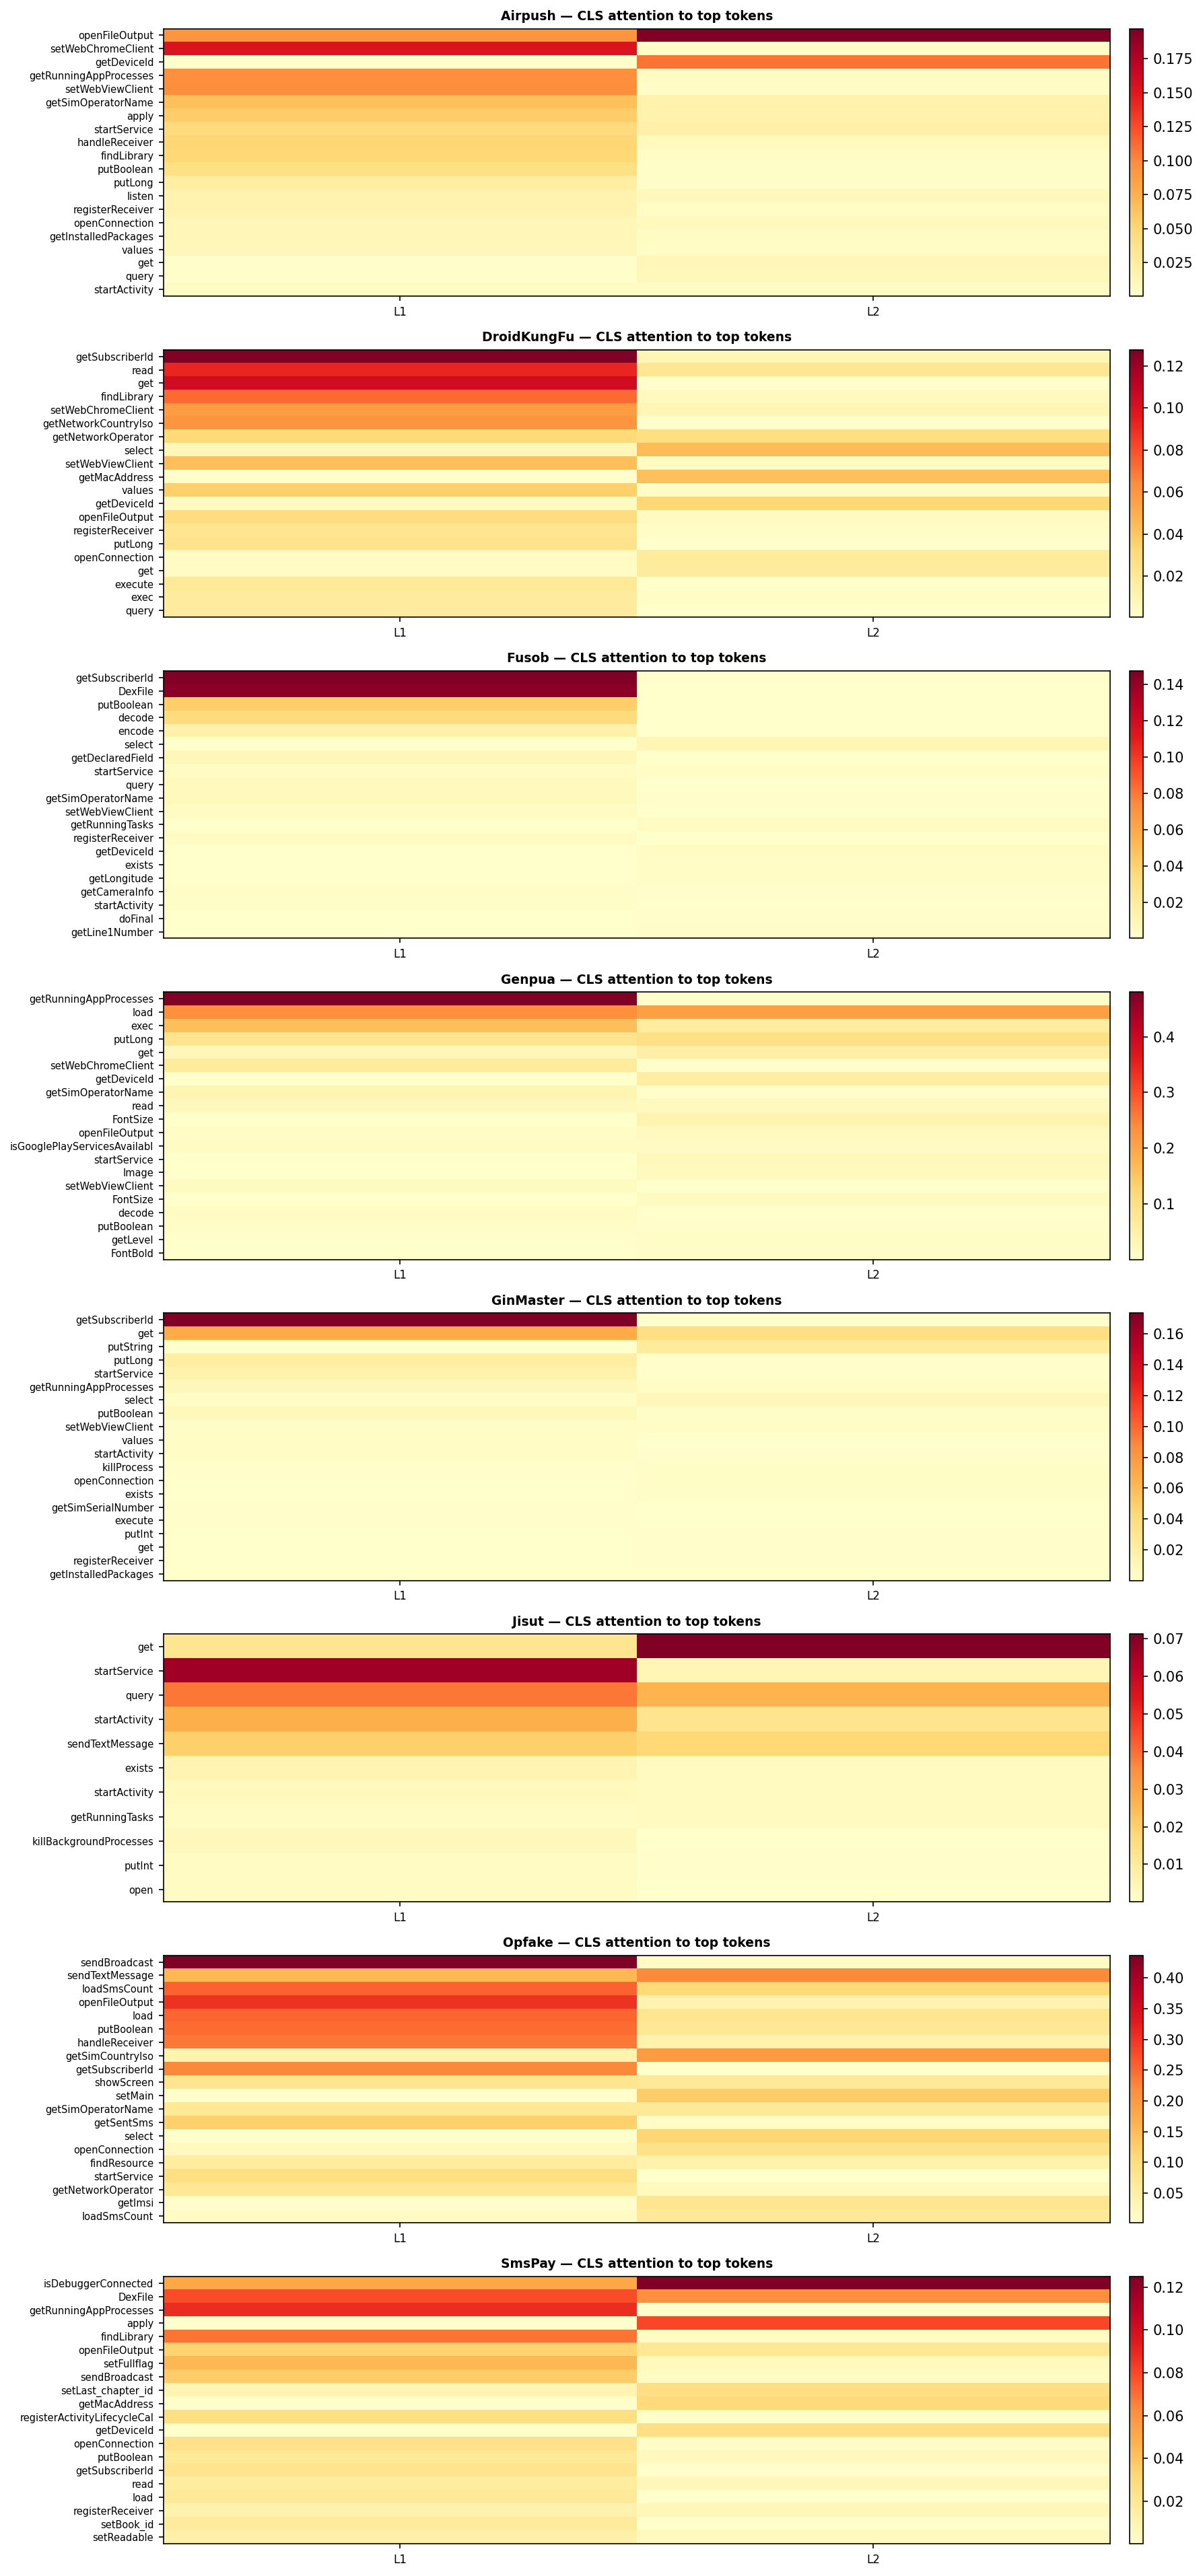
\includegraphics[width=0.48\textwidth]{results/figures/cls_attn_heatmap_per_family.png}
\hfill
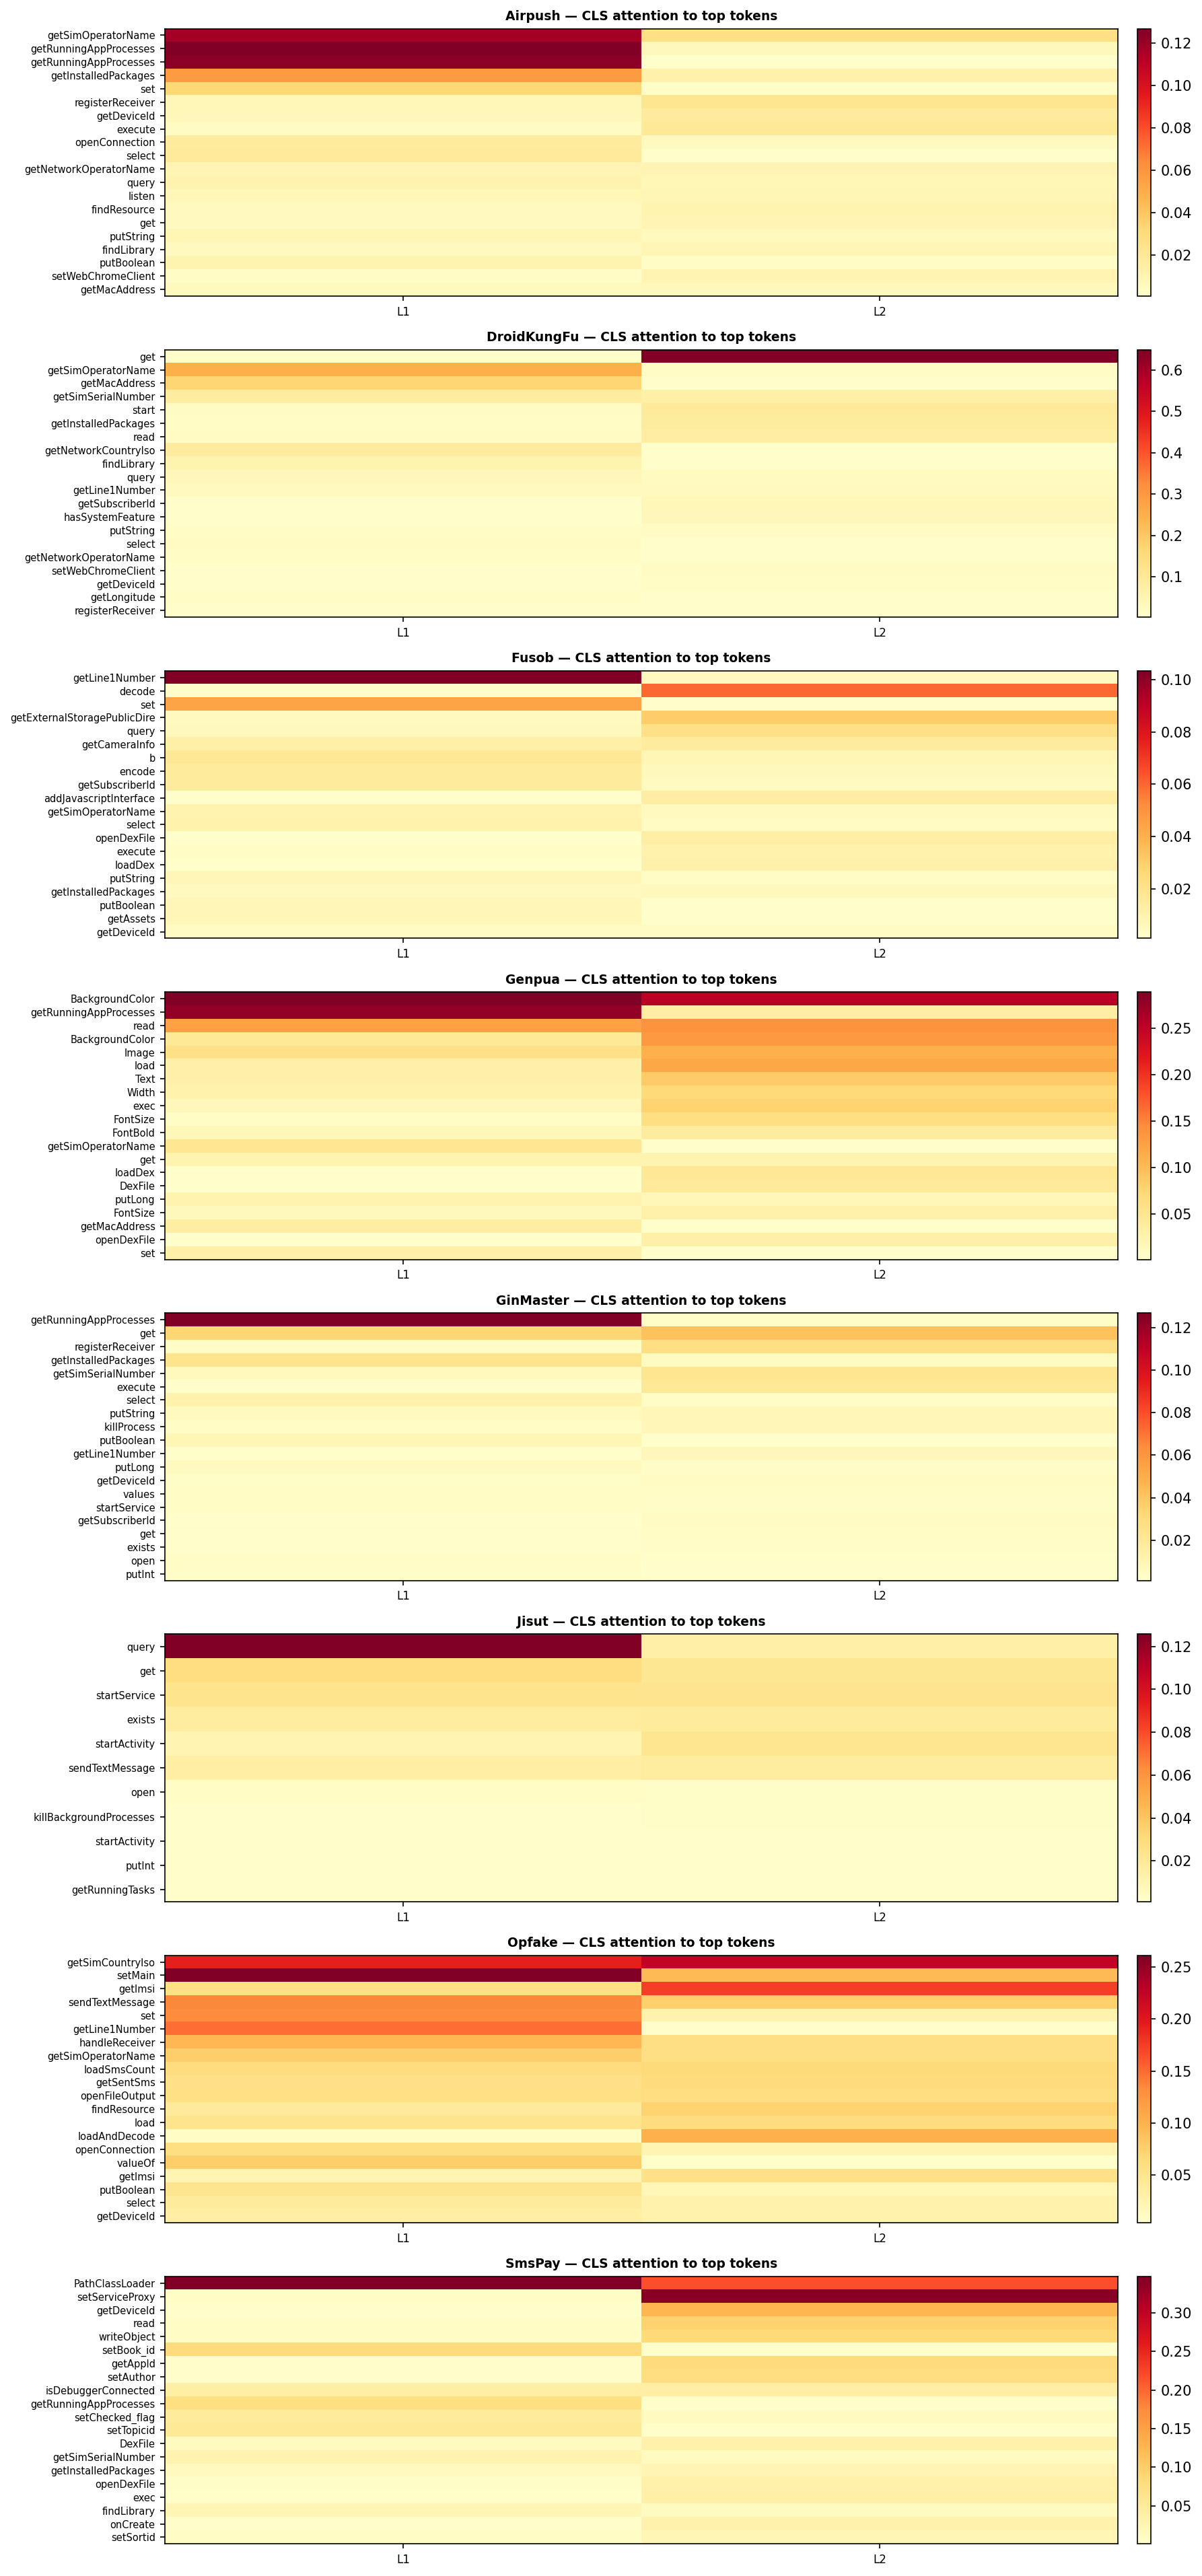
\includegraphics[width=0.48\textwidth]{results/figures/markov_transformer_cls_attn_heatmap_per_family.png}
\caption{Average \textit{[CLS]} attention heatmaps across families for the Plain Transformer (left) and Markov-initialized Transformer (right). The Markov model strongly focuses on specific API chains for families like SmsPay and DroidKungFu, while struggling with parasitic malware like GinMaster where host-app noise dominates the transition matrix.}
\label{fig:attention_heatmaps}
\end{figure*}

\subsection{Classification Performance}

Table~\ref{tab:classification} reports 3-fold stratified CV results for
all models. The Plain Transformer achieves Macro-F1\,=\,0.884, within
1\,pp of the top performer (BiLSTM, 0.894) and comparable to Random
Forest (0.893). It outperforms all other traditional ML baselines by
4--10\,pp in Macro-F1.

The Markov Transformer achieves Macro-F1\,=\,0.858, a 2.6\,pp drop
relative to the plain variant. The structural inductive bias appears
to constrain the model's ability to exploit discriminative patterns
that are not reflected in the global transition structure. We report
this finding honestly: the Markov variant is not a better classifier,
but we show below that its attention tells a more faithful story.

\begin{table}[t]
\centering
\caption{Classification results (3-fold stratified CV, mean\,$\pm$\,std).
  \textbf{Bold}: best; \underline{underline}: second best.}
\label{tab:classification}
\begin{tabular}{lccc}
\toprule
\textbf{Model} & \textbf{Accuracy} & \textbf{Macro-F1} & \textbf{AUROC} \\
\midrule
GaussianNB     & 0.860\,$\pm$\,0.001 & 0.782\,$\pm$\,0.007 & 0.925\,$\pm$\,0.007 \\
Decision Tree  & 0.922\,$\pm$\,0.001 & 0.836\,$\pm$\,0.004 & 0.910\,$\pm$\,0.002 \\
LinearSVM      & 0.923\,$\pm$\,0.001 & 0.844\,$\pm$\,0.009 & 0.980\,$\pm$\,0.005 \\
Markov Trans.  & 0.927\,$\pm$\,0.004 & 0.858\,$\pm$\,0.004 & 0.976\,$\pm$\,0.003 \\
Plain Trans.   & 0.940\,$\pm$\,0.003 & \underline{0.884\,$\pm$\,0.009} & 0.981\,$\pm$\,0.003 \\
BiLSTM         & \textbf{0.948\,$\pm$\,0.004} & \textbf{0.894\,$\pm$\,0.003} & \underline{0.992\,$\pm$\,0.001} \\
Rand.\ Forest  & \underline{0.950\,$\pm$\,0.003} & 0.893\,$\pm$\,0.010 & \textbf{0.993\,$\pm$\,0.001} \\
\bottomrule
\end{tabular}
\end{table}

\subsection{Faithfulness Analysis}
\label{sec:faithfulness}

Table~\ref{tab:faithfulness} reports deletion test results at
$m \in \{5, 10, 20\}$. Both models pass the base faithfulness
criterion ($G > 0$ at all $m$). However, the Markov Transformer
produces markedly larger faithfulness gaps throughout, with the
advantage growing from 0.5\,pp at $m{=}5$ to 10.1\,pp at $m{=}20$.
This indicates that Markov-initialized attention heads identify tokens
the model relies on considerably more precisely than randomly initialized
attention heads at the same architecture and scale.

\begin{table}[t]
\centering
\caption{Deletion test: mean probability drop $\Delta$ when masking top-$m$
  CLS-attention tokens vs.\ $m$ random tokens (240 samples, 8 families).}
\label{tab:faithfulness}
\resizebox{\columnwidth}{!}{%
\begin{tabular}{llccc}
\toprule
\textbf{Model} & \textbf{Metric} & $m{=}5$ & $m{=}10$ & $m{=}20$ \\
\midrule
\multirow{3}{*}{Plain Trans.}
  & $\Delta_{\text{attn}}$  & 9.5\%  & 13.9\%  & 18.7\% \\
  & $\Delta_{\text{rand}}$  & 0.5\%  &  0.6\%  &  1.7\% \\
  & Gap $G$                 & 9.0\%  & 13.3\%  & 17.0\% \\
\midrule
\multirow{3}{*}{Markov Trans.}
  & $\Delta_{\text{attn}}$  & 9.5\%  & 18.3\%  & 27.2\% \\
  & $\Delta_{\text{rand}}$  & 0.01\% &  0.9\%  &  0.1\% \\
  & Gap $G$                 & \textbf{9.5\%} & \textbf{17.4\%} & \textbf{27.1\%} \\
\bottomrule
\end{tabular}%
}
\end{table}

\subsection{Per-Family Faithfulness}

Table~\ref{tab:perfamily} breaks down faithfulness gaps by family at
$m{=}20$. The Markov Transformer outperforms the plain variant in 6 of
8 families.

\begin{table}[t]
\centering
\caption{Per-family faithfulness gap $G$ at $m{=}20$.
  $\uparrow$: Markov $>$ Plain;\; $\downarrow$: Markov $<$ Plain.}
\label{tab:perfamily}
\begin{tabular}{lccc}
\toprule
\textbf{Family} & \textbf{Plain $G$} & \textbf{Markov $G$} & \textbf{Dir.} \\
\midrule
Airpush      &  0.4\% &  16.0\% & $\uparrow$ \\
DroidKungFu  & 26.8\% &  55.2\% & $\uparrow$ \\
Fusob        &  0.0\% &  22.2\% & $\uparrow$ \\
Genpua       & 19.7\% &  30.7\% & $\uparrow$ \\
GinMaster    & 51.9\% &  12.0\% & $\downarrow$ \\
Jisut        &  0.1\% &   0.0\% & $\approx$ \\
Opfake       & 21.1\% &  24.3\% & $\uparrow$ \\
SmsPay       & 15.6\% &  56.8\% & $\uparrow$ \\
\bottomrule
\end{tabular}
\end{table}

\textbf{Sequential structure drives the gain.}
SmsPay (15.6\%\,$\to$\,56.8\%) and DroidKungFu (26.8\%\,$\to$\,55.2\%)
show the largest faithfulness gains. Both families have tight,
well-defined API chains: SmsPay follows a predictable
register\,$\to$\,compose\,$\to$\,send SMS sequence, while DroidKungFu
executes a root-exploit-then-exfiltrate pattern.
These behavioral regularities are well-captured by k-spaced transition
counting, so the corresponding API tokens receive large embedding
norms and attract attention from early in training.
Fusob (ransomware, 0.0\%\,$\to$\,22.2\%) improves substantially for a
different reason: the plain model is probability-saturated
($P_0{>}0.999$) and deletion moves nothing, while the Markov model
retains sensitivity---masking its top-attended tokens causes a
measurable confidence drop, indicating it has learned to rely on
a specific subset of API calls rather than classifying by exclusion.

\textbf{The GinMaster exception.}
GinMaster is the notable outlier (51.9\%\,$\to$\,12.0\%).
GinMaster is a \textit{parasitic} malware that embeds itself inside
legitimate host applications; its API traces are therefore dominated
by host-app behavior---UI lifecycle, I/O, and network calls typical
of benign software. The global Markov transition matrix is shaped by
the majority of non-GinMaster samples, so Markov-initialized embeddings
assign high salience to host-app API patterns rather than to the
small set of characteristic system calls that distinguish GinMaster.
The plain Transformer, unconstrained by this structural prior, learns
to attend directly to those distinguishing calls.
This result highlights an important boundary condition for the method:
when the malware signal is sparse relative to host noise, a global
transition prior can actively mislead attention.

\subsection{Qualitative Attention Analysis}

The deletion test establishes \textit{that} the Markov model's
attention is more faithful; inspecting the attention distribution
reveals \textit{why} (see Fig.~\ref{fig:attention_heatmaps}).


For families with tight, sequential API chains, the Markov model
concentrates attention on a small cluster of high-transition-weight
tokens. In SmsPay, a consistent focus on telephony management and
SMS dispatch APIs emerges across test samples. These APIs form the
core register\,$\to$\,compose\,$\to$\,send chain and that appear
as high-weight edges in the global transition matrix. Masking just
these 20 tokens collapses model confidence by over 56\,pp
(Table~\ref{tab:perfamily}), confirming this cluster is genuinely
load-bearing.

For DroidKungFu, the Markov model attends strongly to privilege
escalation and network I/O APIs, reflecting the exploit\,$\to$\,exfiltrate
chain encoded by multi-hop transitions. The plain Transformer, by
contrast, distributes attention more broadly across the sequence:
many weakly relevant tokens each receive moderate attention, but
removing any small subset causes only a mild confidence drop. This
diffuse pattern is mechanistically consistent with the plain model's
lower faithfulness gap, as it has learned to classify from the overall
statistical profile of the sequence rather than from a small set of
critical API calls.

The contrast is sharpest for GinMaster. The Markov model's attention
is dominated by common host-application APIs (activity lifecycle,
I/O, UI events) that appear frequently in the training corpus and
thus form high-weight transition edges. However, these APIs are shared
with benign software and carry no discriminative signal for GinMaster.
The plain Transformer, learning purely from gradient signal, attends
to the small set of system calls that distinguish GinMaster from its
host, achieving a substantially higher faithfulness gap (51.9\%
vs.\ 12.0\%). This contrast is the clearest illustration of the
structural prior as a double-edged constraint: it sharpens attention
when global transition structure aligns with the discriminative signal,
and degrades it when that structure is dominated by irrelevant patterns.

\subsection{Discussion}

\textbf{Accuracy--explainability tradeoff.}
Markov initialization acts as a structural regularizer: it constrains
the embedding space to reflect transition dynamics, reducing the model's
freedom to exploit spurious statistical correlations that boost accuracy
but produce unfaithful explanations. This tradeoff is a meaningful
design decision in practice. In high-stakes deployment scenarios such
as forensic analysis or legal attribution, where the explanation must
be defensible, a model with more faithful attention may be preferred
even at a small accuracy cost.

\textbf{Limitations.}
Results are on a single corpus with 8 families; generalization to other
datasets (Drebin, CICAndMal2017) or to unseen families is untested.
Fusob and SmsPay ($\leq$173 samples each) have few test examples per
fold, making per-class metrics for these families noisy.
Vocabulary is constructed before fold splitting---a soft leakage of
token existence (but not label information) that is documented but
not resolved.
Finally, the deletion test is a necessary but not sufficient condition
for faithfulness: $G > 0$ does not guarantee that the attention map is
complete or causally faithful as an explanation.

% ─────────────────────────────────────────────────────────────────────────────
\section{Conclusion}

We proposed Markov-initialized Transformer embeddings for explainable
Android malware family classification. SVD factorization of k-spaced
API transition matrices encodes global behavioral structure into the
embedding layer prior to training. A rigorous deletion-based faithfulness
test on 9,337 Droidmon traces shows that this initialization produces
\textit{[CLS]} attention maps that are more tightly coupled to model
behavior than those of a plain Transformer, with faithfulness gap
27.1\% vs.\ 17.0\% at $m{=}20$. This improvement comes at a 2.6\,pp
Macro-F1 cost, exposing a real accuracy--explainability tradeoff.
The per-family analysis reveals that the benefit is tied to behavioral
structure: families with stereotyped API sequences benefit most. However, we explicitly note that when malware signal is sparse relative to host noise (as seen with the parasitic GinMaster family), the global transition prior can actively mislead attention and hinder explainability, highlighting an important boundary condition for this approach.

Future work includes per-class or pseudo-label-conditioned transition
matrices, PPMI normalization of $\mathbf{T}$ prior to SVD, and
validation on additional corpora to test whether the faithfulness
improvement generalizes beyond this dataset.

% ─────────────────────────────────────────────────────────────────────────────
\bibliographystyle{IEEEtran}

\begin{thebibliography}{00}

\bibitem{av_test_2023}
AV-TEST Institute, ``Malware statistics \& trends report,''
\textit{av-test.org}, 2023.

\bibitem{lundberg2017shap}
S.~M. Lundberg and S.-I. Lee,
``A unified approach to interpreting model predictions,''
in \textit{Proc. NeurIPS}, 2017, pp.\ 4765--4774.

\bibitem{jain2019attention}
S.~Jain and B.~C. Wallace,
``Attention is not explanation,''
in \textit{Proc. NAACL-HLT}, 2019, pp.\ 3543--3556.

\bibitem{wiegreffe2019attention}
S.~Wiegreffe and Y.~Pinter,
``Attention is not not explanation,''
in \textit{Proc. EMNLP-IJCNLP}, 2019, pp.\ 11--20.

\bibitem{samek2017evaluating}
W.~Samek, A.~Binder, G.~Montavon, S.~Lapuschkin, and K.-R. M\"{u}ller,
``Evaluating the visualization of what a deep neural network has learned,''
\textit{IEEE Trans.\ Neural Netw.\ Learn.\ Syst.}, vol.\ 28, no.\ 11,
pp.\ 2660--2673, 2017.

\bibitem{abnar2020rollout}
S.~Abnar and W.~Zuidema,
``Quantifying attention flow in Transformers,''
in \textit{Proc. ACL}, 2020, pp.\ 4190--4197.

\bibitem{sundararajan2017integrated}
M.~Sundararajan, A.~Taly, and Q.~Yan,
``Axiomatic attribution for deep networks,''
in \textit{Proc. ICML}, 2017, pp.\ 3319--3328.

\bibitem{dangelo2023kspaced}
G.~D'Angelo, F.~Palmieri, and S.~Robustelli,
``k-Spaced associative classification rules for mobile malware detection,''
\textit{Expert Syst.\ Appl.}, 2023.

\bibitem{nataraj2011malware}
L.~Nataraj, S.~Karthikeyan, G.~Jacob, and B.~S. Manjunath,
``Malware images: Visualization and automatic classification,''
in \textit{Proc. VizSec}, 2011, pp.\ 1--7.

\bibitem{ye2019deep}
Y.~Ye, T.~Li, D.~Adjeroh, and S.~S. Iyengar,
``A survey on malware detection using data mining techniques,''
\textit{ACM Comput.\ Surv.}, vol.\ 50, no.\ 3, pp.\ 41:1--41:40, 2017.

\bibitem{vaswani2017attention}
A.~Vaswani et al.,
``Attention is all you need,''
in \textit{Proc. NeurIPS}, 2017, pp.\ 5998--6008.

\bibitem{pennington2014glove}
J.~Pennington, R.~Socher, and C.~D. Manning,
``GloVe: Global vectors for word representation,''
in \textit{Proc. EMNLP}, 2014, pp.\ 1532--1543.

\bibitem{mikolov2013word2vec}
T.~Mikolov, I.~Sutskever, K.~Chen, G.~Corrado, and J.~Dean,
``Distributed representations of words and phrases and their compositionality,''
in \textit{Proc. NeurIPS}, 2013, pp.\ 3111--3119.

\bibitem{droidmon}
idanr1986, ``Droidmon - API monitor for Dalvik,''
GitHub repository, 2014. [Online].
Available: \url{https://github.com/idanr1986/droidmon}

\bibitem{hochreiter1997lstm}
S.~Hochreiter and J.~Schmidhuber,
``Long short-term memory,''
\textit{Neural Comput.}, vol.\ 9, no.\ 8, pp.\ 1735--1780, 1997.

\bibitem{breiman2001rf}
L.~Breiman,
``Random forests,''
\textit{Mach.\ Learn.}, vol.\ 45, no.\ 1, pp.\ 5--32, 2001.

\bibitem{soi2024enhancing}
D.~Soi, A.~Sanna, D.~Maiorca, and G.~Giacinto,
``Enhancing Android malware detection explainability through function call graph APIs,''
\textit{Journal of Information Security and Applications}, vol.\ 80, p.\ 103691, 2024.

\bibitem{wu2021why}
T.~Wu, J.~Liu, et al.,
``Why an android app is classified as malware: Toward malware classification interpretation,''
\textit{ACM Trans.\ Softw.\ Eng.\ Methodol.\ (TOSEM)}, 2021.

\bibitem{drebin2014}
D.~Arp, M.~Spreitzenbarth, M.~Hubner, H.~Gascon, and K.~Rieck,
``Drebin: Effective and explainable detection of android malware in your pocket,''
in \textit{NDSS}, 2014.

\bibitem{lashkari2018cicandmal2017}
A.~H. Lashkari et al.,
``Toward developing a systematic approach to generate benchmark android malware datasets and classification,''
in \textit{IEEE ICCST}, 2018.

\end{thebibliography}

\end{document}
